\label{Appendix}
\section{Email to Participants}
\label{Appendix:Email}
Subject: VR Study Participation and Consent

\textit{Consent form}

Dear Participant,

I would like to confirm your participation in my study on $<$Date$>$ at $<$Time$>$. Below is a consent form for the study. Please read and reply with your consent as per the instructions. Below the consent form is a list of requirements for the study.

\textbf{This is a consent form for the Social VR project pilot study.}

In my project I have developed tools for navigating in a virtual environment. In this study I want to determine how effective these tools are for navigating and understanding an environment.

During this study you will be asked to carry out two Tasks. Each task will be of maximum 10 minutes and 10 minute breaks for answering some questions after each task. You will also have some final questions to answer at the end of the study. Participation would take about 50 minutes.

I would like permission to:

\begin{itemize}
	\item Record input from your microphone and tracking sensors.
	\item Record the video of your VR view.
	\item Get some data of your movement within the application.
	\item Get your answers to some questions in a questionnaire.
\end{itemize}

I will anonymize and store this recorded data and the answers to the questionnaire for further analysis to be published in my project report.

Please, inform me immediately if you are feeling unwell during the study process and want to take a break or stop.

You are free to leave the study at any time.

Please reply with your agreement as follows:

I, $<$Name$>$, agree to participation in a user study and the recoding of my data following the above conditions

\textbf{Requirements List}

To be able to participate please follow the steps outlined below prior to the study time:

\begin{itemize}
	\item Make sure that you will not be disturbed for the time of the study.
	\item Prepare to be standing for the duration that you are in VR (except for breaks).
	\item Make sure you are following all Covid guidelines when coming to the location of the study.
\end{itemize}

The following details are the location of the study Please be here at least 5 minutes before the start time:

$<$Location$>$

Thank you for your participation. Please email me if you have any concerns or questions

Regards,

Ramsha Saad Thaniana

\section{Questionnaire}
\label{Appendix:Questionnaire}
The following are the questions that were in the questionnaire given to participants in the user study. Questions asked after each task were specific to the task and can be divided into questions on user comfort, task load and comprehensibility of jumps. There were also some end of study questions.
\subsection{User Comfort}
\begin{itemize}
	\item On a scale of 0 to 10, 0 being how you felt coming in, 10 is that you want to stop, where are you now?\\
	\textit{Answered on a discrete scale from 0 (How you felt coming in) to 10 (You want to stop)}
	\item How comfortable were you during the task? coming in, 10 is that you want to stop, where are you now?\\ 
	\textit{Answered on a discrete scale from 0 (Not comfortable) to 10 (Very comfortable)}
	\item Please explain the reasons for the level of comfort that you chose above.\\
	\textit{Answered on a free text field}
\end{itemize}
\subsection{Task Load}
The electronic version of the \acrfull{rtlx} questionnaire had the following questions that have to be answered on a scale of 0 to 100 in steps of 5 with a slider and numbers hidden to the participant. 
\begin{itemize}
	\item Mental Demand - How mentally demanding was the task?\\
	\textit{0 (Very Low) to 10 (Very High)}
	\item Physical Demand - How physically demanding was the task?\\
	\textit{0 (Very Low) to 10 (Very High)}
	\item Temporal Demand - How hurried or rushed was the pace of the task?\\
	\textit{0 (Very Low) to 10 (Very High)}
	\item Performance - How successful were you in accomplishing what you were asked to do?\\
	\textit{0 (Perfect) to 10 (Failure)}
	\item Effort - How hard did you have to work to accomplish your level of performance?\\
	\textit{0 (Very Low) to 10 (Very High)}
	\item Frustration - How insecure, discouraged, irritated, stressed and annoyed were you?\\	
	\textit{0 (Very Low) to 10 (Very High)}
\end{itemize}
\subsection{Comprehensibility of Jumps}
\begin{itemize}
	\item How were you getting to the next position?\\
	\textit{Answered on a free text field}
	\item How often were you confused about what your next position would be?\\
	\textit{Answered on a discrete scale from 0 (Never) to 10 (At every jump)}
	\item How did you know what your next position would be?\\
	\textit{Answered on a free text field}
	\item How often were you confused about what direction you would be facing after a jump?\\
	\textit{Answered on a discrete scale from 0 (Never) to 10 (At every jump)}
	\item How did you know what direction you would be facing after a jump?\\
	\textit{Answered on a free text field}
	\item If you have mentioned that you were confused about your next position/direction please explain what you were confused about.\\
	\textit{Answered on a free text field}
	\item Were you confused about anything else? If so what were you confused about?\\
	\textit{Answered on a free text field}
	\item Do you have anything more to add for this task?\\
	\textit{Answered on a free text field}
\end{itemize}
\subsection{Final Questions}
For these questions participants were aware that Task A refers to the task they did first and Task B refers to the task that they did second.
\begin{itemize}
	\item Which method did you prefer?\\
	\textit{Answered by choosing an option from the options (Task A, Task B)}
	\item Why did you prefer this method?\\
	\textit{Answered on a free text field}
	\item Can you think about any scenario in which you would prefer to use the method in Task A for?\\
	\textit{Answered on a free text field}
	\item Can you think about any scenario in which you would prefer to use the method in Task B for?\\
	\textit{Answered on a free text field}
	\item What did you like about the method in Task A?\\
	\textit{Answered on a free text field}
	\item What did you like about the method in Task B?\\
	\textit{Answered on a free text field}
	\item Do you have anything more to add about the method in Task A?\\
	\textit{Answered on a free text field}
	\item Do you have anything more to add about the method in Task B?\\
	\textit{Answered on a free text field}
	\item Any final comments?\\
	\textit{Answered on a free text field}
\end{itemize}
\section{Maps for Path Recall}
\label{Appendix:Path Recall}
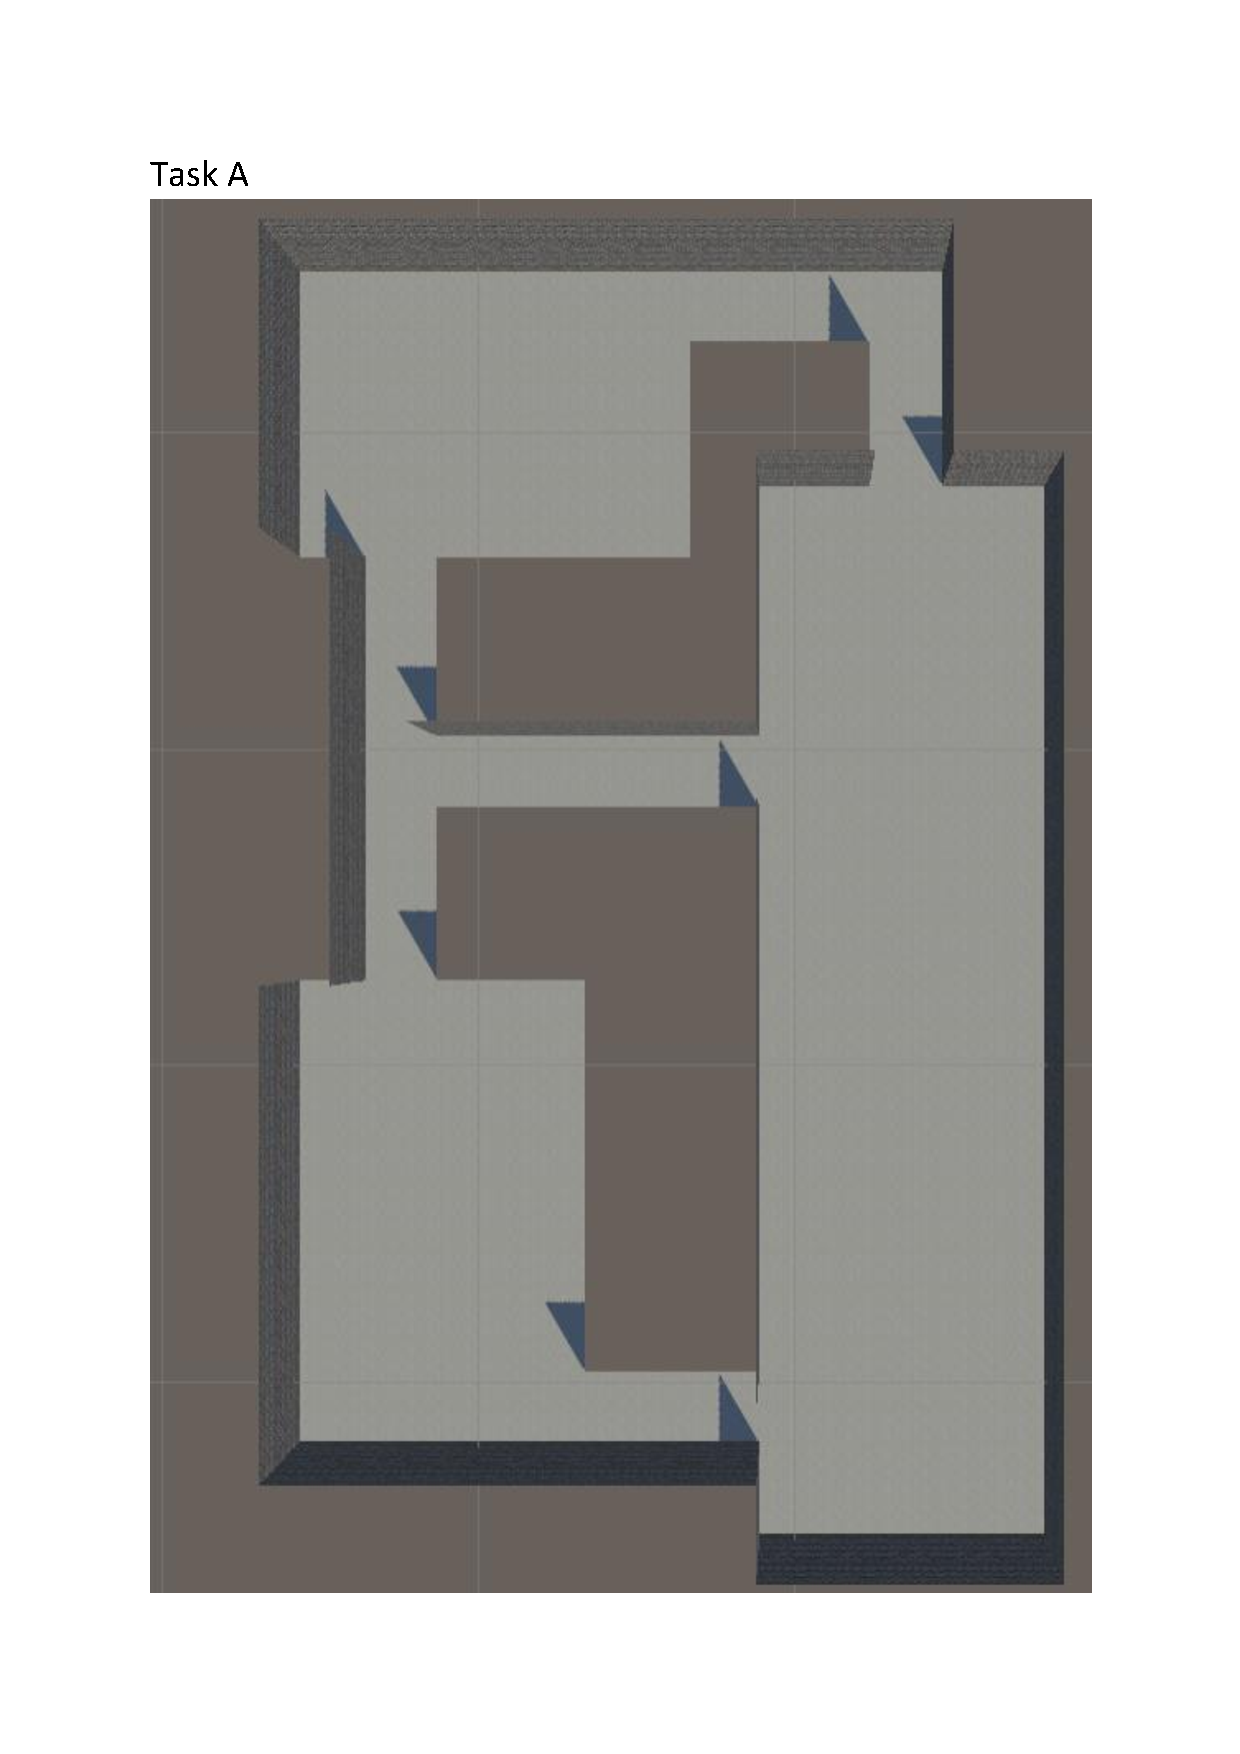
\includepdf[scale=0.9,pages=1-2,pagecommand={\thispagestyle{myheadings}}]{appendix/Maps.pdf}
\label{Appendix:Sample Logging Data}
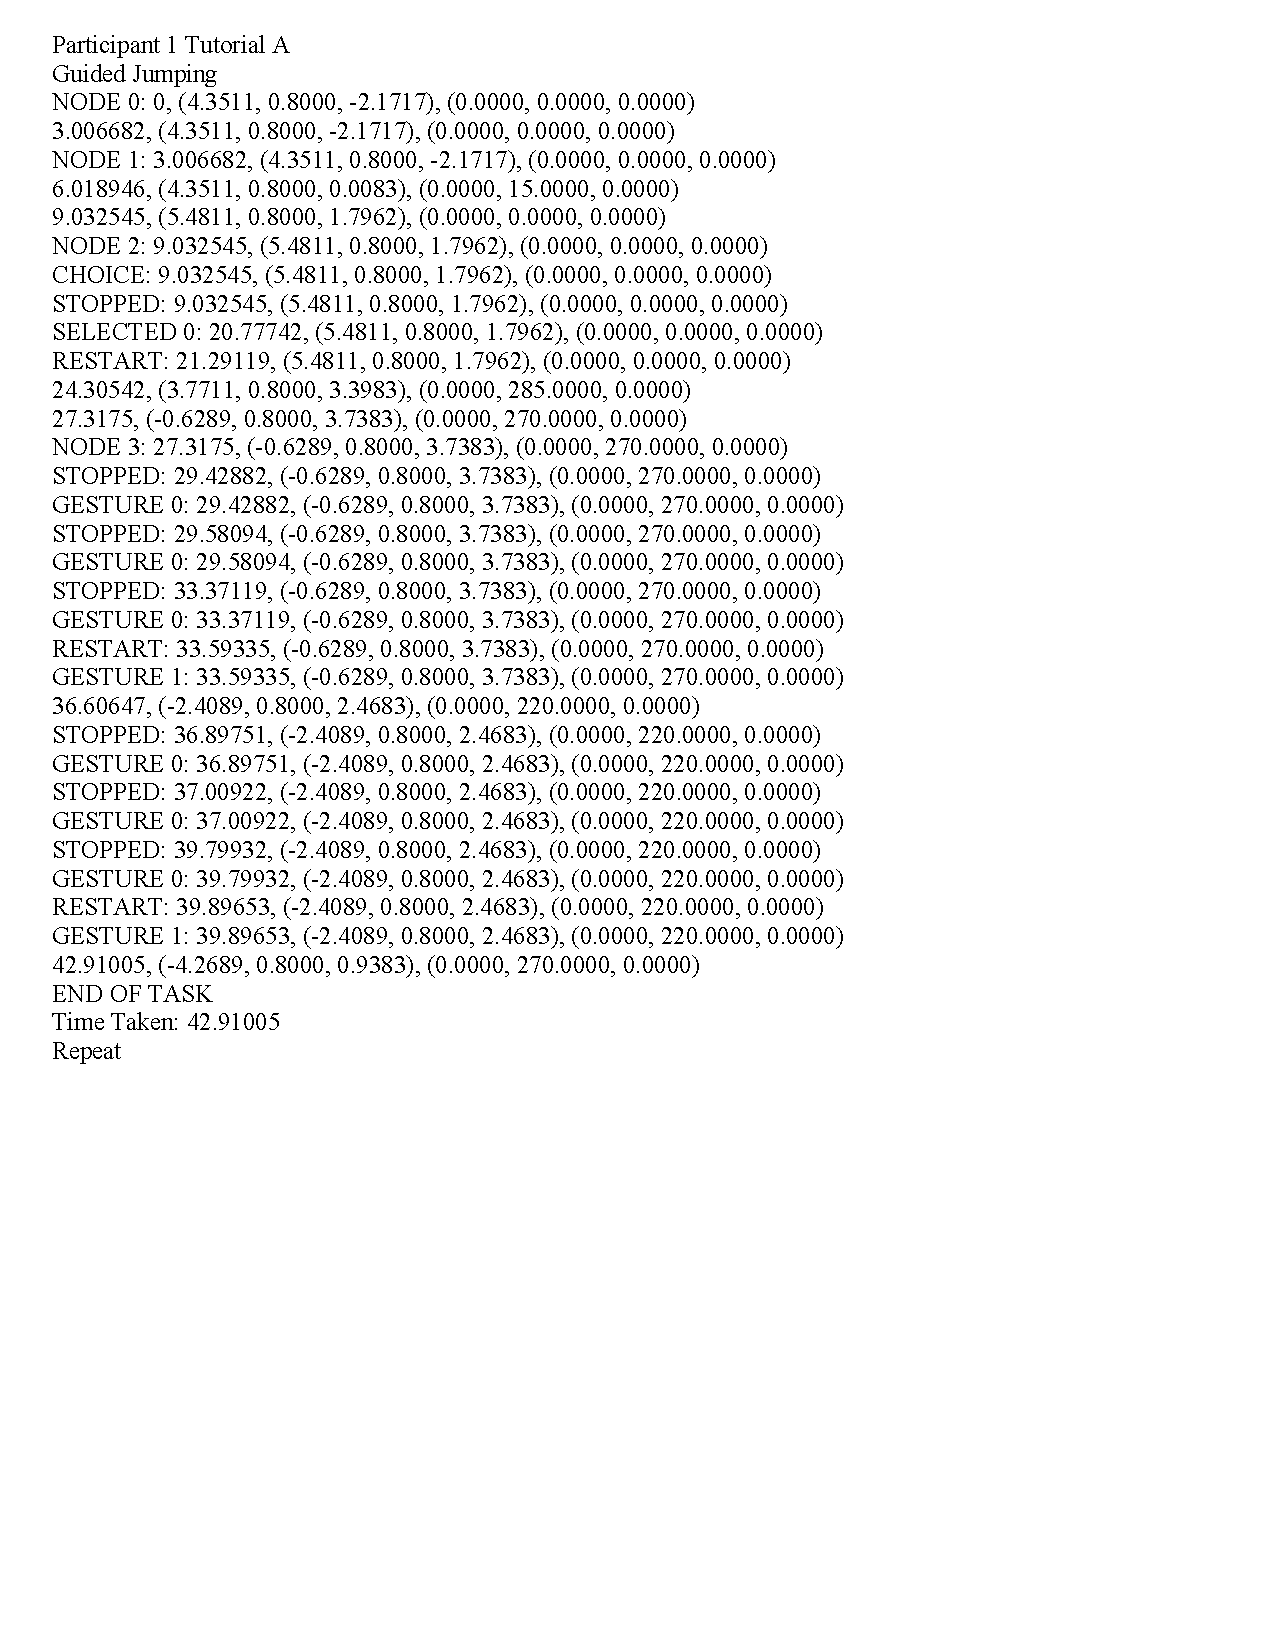
\includepdf[scale=0.9,pages=1,pagecommand={\thispagestyle{myheadings}},pagecommand={\section{Sample Logging Data}}, offset=0 -2cm]{appendix/sample-logging-automated.pdf}
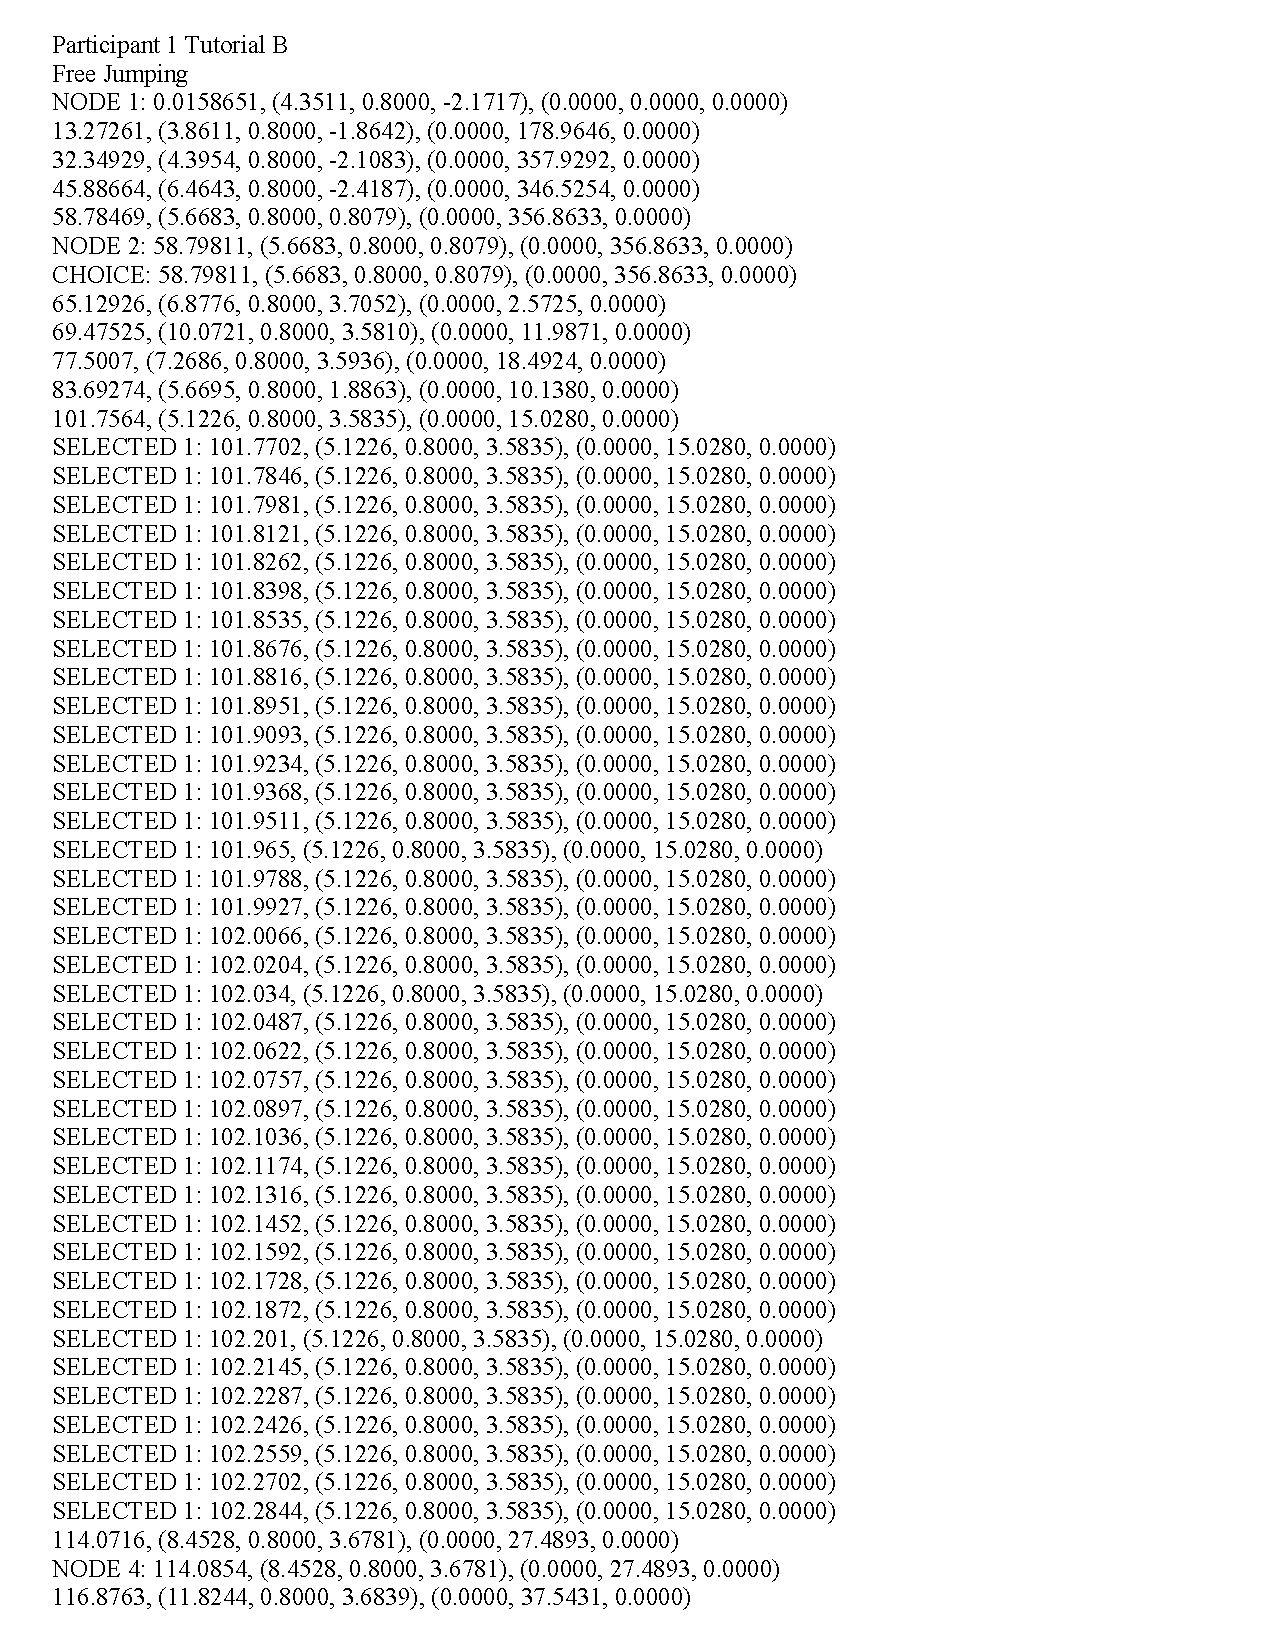
\includepdf[scale=0.9,pages=1,pagecommand={\thispagestyle{myheadings}}]{appendix/sample-logging-free.pdf}